\documentclass[a4paper,11pt,french]{article}

\usepackage[frenchb]{babel}
\usepackage[T1]{fontenc}
\usepackage[utf8]{inputenc}
\usepackage{um2/um2}
\usepackage{verbatim}
\usepackage{graphicx}


\setlength{\parindent}{0pt}
\setlength{\parskip}{2ex}


\title{Rapport de TER\\---\\Reconception du jeu Pticlic sous Android}
\author{Yoann \textsc{Bonavero} \and Bertrand \textsc{Brun} \and John \textsc{Charron} \and Georges \textsc{Dupéron}}

\begin{document}

\maketitle


\pagestyle{empty}
\thispagestyle{empty}

\tableofcontents


\pagestyle{empty}
\thispagestyle{empty}
\newpage
\setcounter{page}{1}
\pagestyle{plain}


\section{Introduction}

PtiClic\footnote{http://pticlic.org} est un jeu qui a été conçu et développé par Matthieu Lafourcade et Virginie Zampa. Le jeu a été créé afin de faire des études sur le vocabulaire et la sémantique sur des sujets de divers horizons dans un contexte ludique et motivant. Un mot central apparait, un nuage de mots entoure le mot central et le joueur clique et dépose des mots du nuage dans des catégories proposé sous forme d'énoncés. 

Par exemple, pour le mot central 'bicyclette', les mots 'pédale', 'piéton', 'pied', 'automobile', 'Sébastien Chabal', 'Lance Armstrong', 'pédalier', 'voiture', 'yeux', 'rapide', 'routier', 'maillot', 'pédaler', 'dopage', 'véhicule', 'musclé', 'nez', etc. sont proposé. Le joueur dépose ces mots dans les catégories "... est une partie de 'cycliste', "Un contraire de 'cycliste' est ...", "'cycliste' a un rapport avec ...",  "Une caractéristique de 'cycliste' est ..." ou aucune de ces catégorie. Un score est obtenu en soustrayant les mots manquants et les mots incorrects des mots corrects. 

Des linguistes et des informaticiens récupèrent les données liées aux parties jouées, ce qui leur permet de faire de la recherche dans leurs domaines respectifs.

Notre travail consiste à créer une version du PtiClic sous Android, une version modifiée du jeu adaptée pour téléphone mobile. Le sujet du TER définit clairement l'objectif de ce projet~:

\begin{quotation}
%% Correction Bertarnd remplacement de fonctionnant sur des Android semble est intéressante => fonctionnant sur Android semble intéressante => NON, CAR CITATION, ON NE PEUT PAS LE 'CORRIGER'
L'étude et le prototypage d'une version fonctionnant sur Android semble intéressante. En particulier on s'intéressera a deux aspects : * les contraintes imposées par l'environnement smartphone * le biais qu'imposent ces contraintes sur le jeu et les données récoltées. Il s'agira donc de modéliser une version adaptée aux smartphones et d'en implémenter un prototype fonctionnel. 
\end{quotation}

Dans un premier temps, une version de base sera conçue et réalisée. Ensuite, des fonctionnalités supplémentaires seront ajouter. La démarche adoptée par notre groupe est une approche itérative. Les quatres livraisons vont d'une version de base vers des versions plus élaborées~: un joueur pourrait, entre autres, modifier ses préférences ou choisir son niveau. L'idée est aussi de rendre le jeu plus attirant afin d'accroître le nombre de sujets participant aux études liées au résultat des données extraits des parties jouées.


\subsection{Android}

Android est un système d'exploitation pour téléphone mobile basé sur le noyau Linux développé par Android Inc., racheté par Google en 2005. Google et d'autres membres du Open Handset Alliance ont par la suite contribué à son développement et le Android Open Source Project (AOSP) est chargé de la maintenance et l'évolution d'Android. Ce système d'exploitation est utilisé notamment dans des smartphones, appelé aussi ordiphones, 'terminaux de poche' ou 'téléphones intelligents', produits et distribués par un grand nombre de fabriquants de téléphones mobiles. Le nombre de téléphones mobiles intégrant le système d'exploitation d'Android a cru sensiblement récemment.

Un grand nombre de développeurs ont créés des applications pour étendre la fonctionnalité des téléphones sous Android et il y a aujourd'hui plus de 200 000 applications disponibles. Bien qu'Android Market est le magasin en ligne opéré par Google, il existe d'autres distributeurs d'applications Android. La majorité des applications sont écrites en Java, bien qu'il soit possible de développer des applications en Python, en Ruby et d'autres par le biais du Android Scripting Environment. 

 
\section{Analyse de l'existant}

L'application du jeu du PtiClic d'origine est une application disponible en ligne sur http://www.lirmm.fr/pticlic/pticlic.php. Nous n'avions pas accès au code source de l'application ni à des diagrammes UML. La seule partie de cette application qui nous a été fournie est le dump de la base de données. 

L'analyse de l'existant consistait donc d'une analyse du dump de la base de données ainsi que l'application sur Internet que nous avons testé et analysé.

\subsection{Le déroulement du jeu}
L'utilisateur clique sur le boutont \"Je joue !\". Un mot se dirige vers le centre de la page , c'est mot central. D'autres mots viennent entourer le mot central, ce sont les mots nuage. La police du mot central est plus grande que celle des mots nuages. Le mot central et les mots nuages sont sont de couleurs contrastées.

\begin{center}
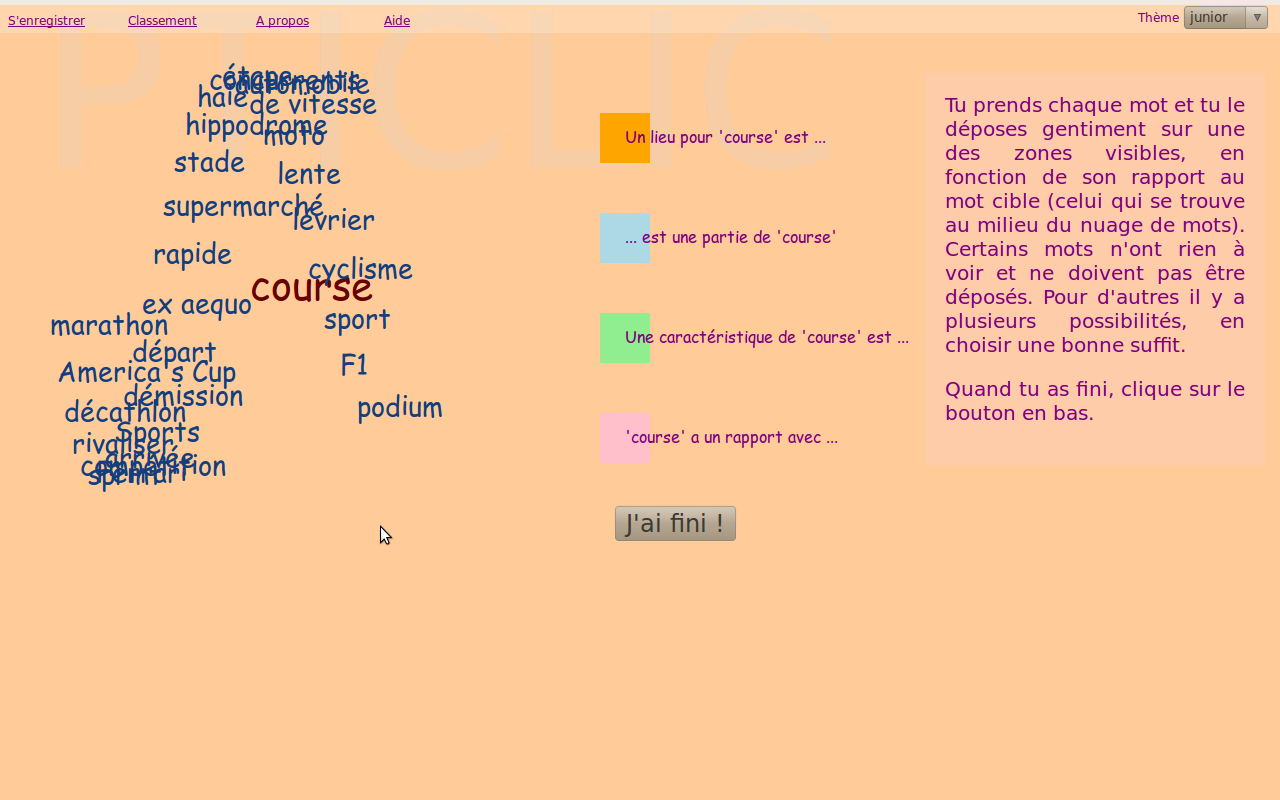
\includegraphics[width=14cm]{img/PtiClicJeu.png}
\end{center}

Les relations apparaît à droite des mots. Une partie peut comporter de un à quatre relations. Un carré apparaît à droite de la relation suivi de la relation sous forme de syntagme tel que \"(mot central) est en rapport avec...\", \"Quoi/Qui pourrait (mot central)~?\". S'il y a plus d'une relation, les relations apparaîssent les unes en dessous les autres, toujours à droite de l'espace mots.

Encore plus à droite, un bref explicatif du principe du jeu, et tout en bas, le bouton \"J'ai fini~!\", 

Le principe du jeu est simple. Lorsque l'utilisateur estime qu'un mot nuage est lié au mot central par une des relations, il glisse et dépose le mot nuage sur le carré de la relation. Si l'utilisateur pense qu'aucune des relations convient, il laisse le mot dans le nuage tout simplement. 

\begin{center}
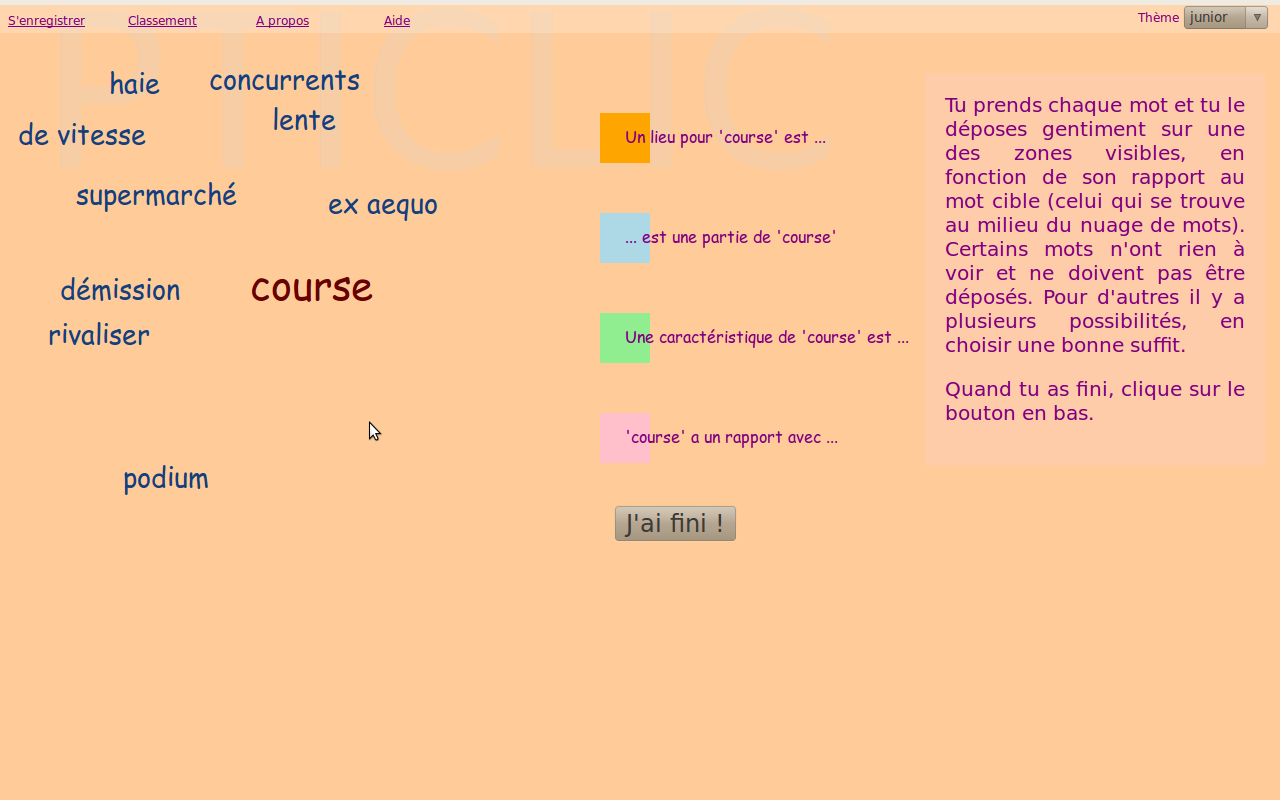
\includegraphics[width=14cm]{img/PtiClicJeu2.png}
\end{center}

Si le joueur se trompe, il peut double-cliquer sur le carré pour extraire le dernier mot déposé. En fait, le joueur peut double-cliquer autant de fois qu'il le veut pour extraire tous les mots ayant été mis dans la relation un par en afin de modifier ses choix. Lorsque le joueur a fait ses choix et souhaite finir sa partie, il clique sur \"J'ai fini !\", ce qui renvoie vers la page des résultats et du score. Il n'y a aucune limite de temps pour jouer ce jeu.

\begin{center}
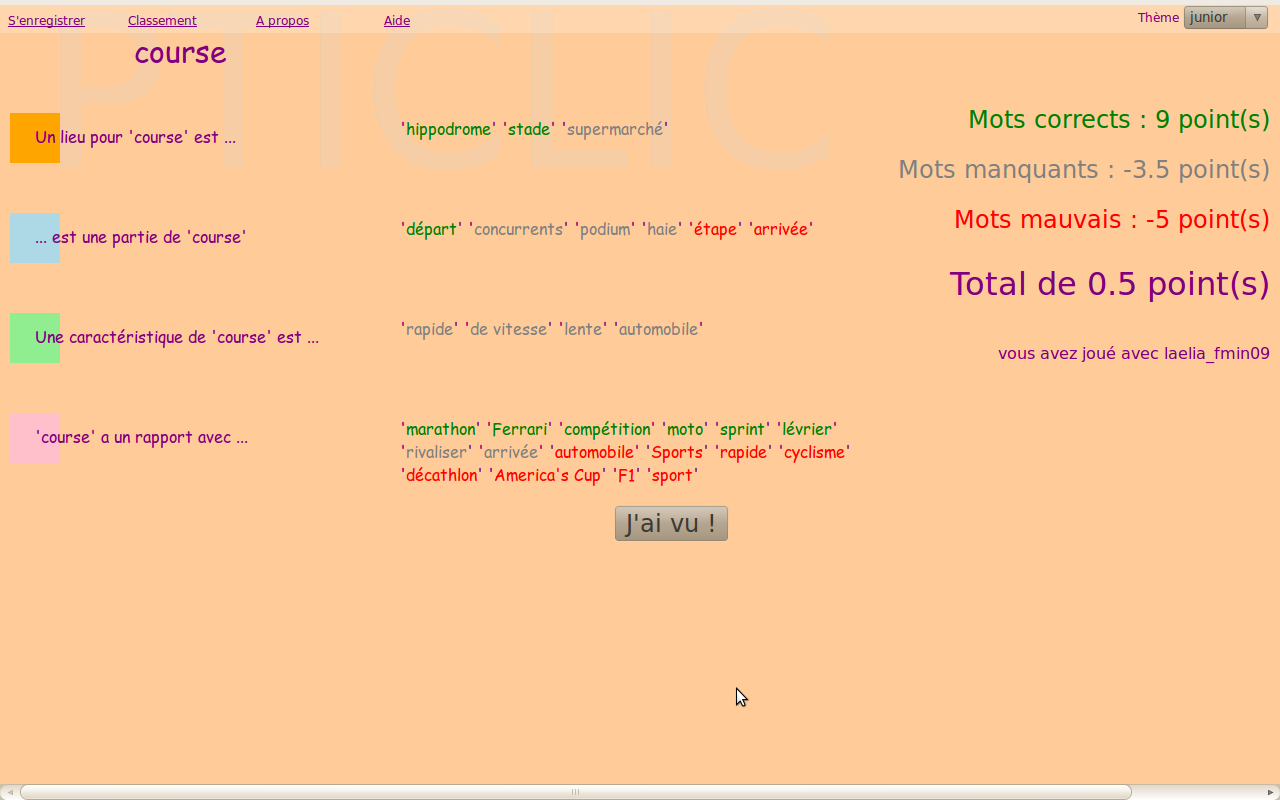
\includegraphics[width=14cm]{img/PtiClicResultats.png}
\end{center}

La page des scores contient aussi le corrigé de la partie. Les mots qui ont été mis dans la bonne catégories apparaissent en vert, les mauvaises réponses en rouge et les omissions en gris. On marque un point pour les bonnes réponses, on perd un demi point our une mauvaise réponse, on perd un demi-point pour une omission. Lorsque deux réponses sont possibles, on marque un point quelque soit la relation choisie. Le score final est soit un entier, un entier plus un demi point. Le score final peut être négatif, zéro ou positif. 

Lorsque l'on clique sur le bouton \"J'ai vu !\", on retourne sur la page d'accueil :

\begin{center}
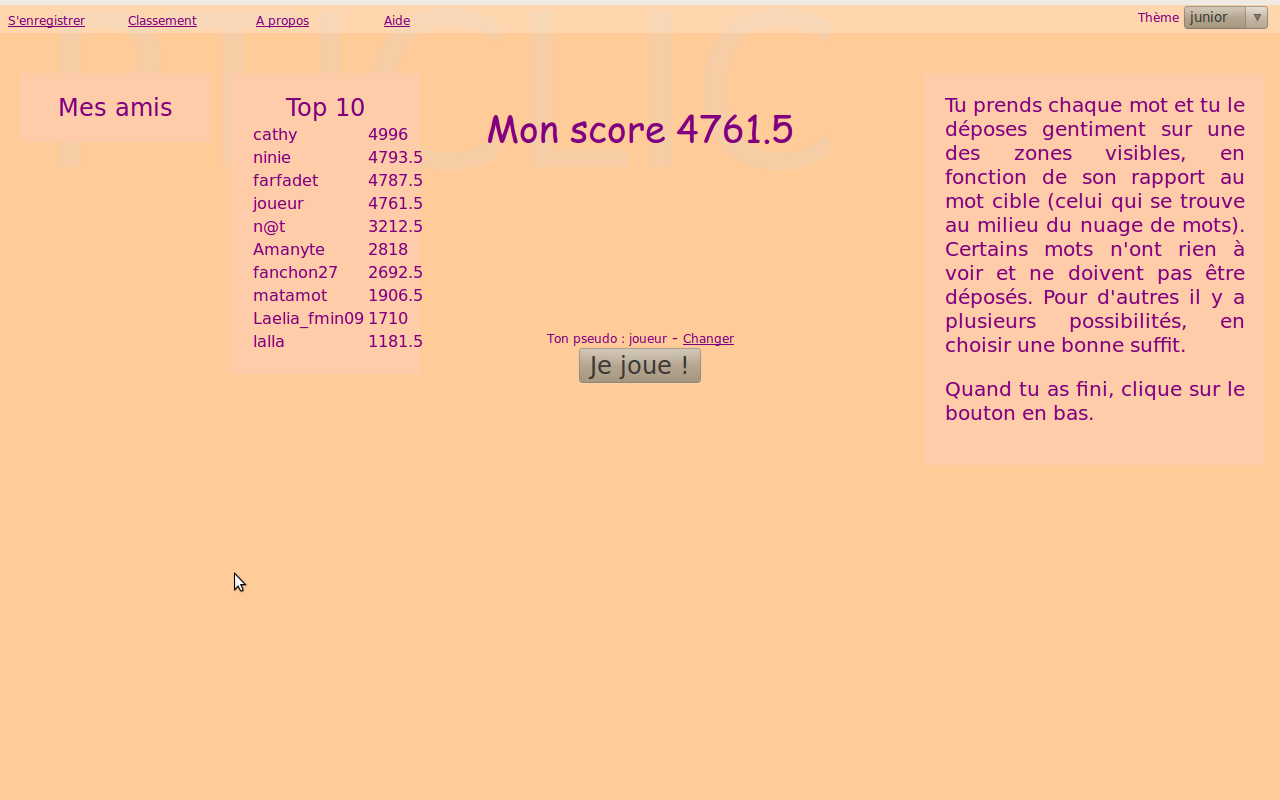
\includegraphics[width=14cm]{img/PtiClicAccueil.png}
\end{center}

Le joueur par défaut est l'utilisateur "joueur". Il est aussi possible de s'inscrire sur le site afin de créer son propre identifiant et mot de passe afin de cumuler des points à chaque fois que l'on joue. Les dix joueurs qui ont cumulé les plus grand nombre de points sont inscrit sur la liste des \"Top 10\". Les points cumulés par le joueur "joueur", qui est l'ensemble de parties jouées par des internautes non inscrits au site, figure parmi les \"Top 10\". A droite de ceci, le score du joueur en question, c'est-à-dire, la somme totale des scores de toutes les parties jouées par l'utilisateur. Si l'utilisateur veut jouer encore une partie, il clique sur le bouton \"Je joue !\" en bas de la page et une nouvelle partie est entamée.

Huit styles de couleurs sont disponible et modifiable dans le menu déroulant en haut et à droite de la page d'accueil. Lorsque le joueur s'authifie avec succès, son identifiant apparaît dans le fond de page en très grande taille.

TODO: MES AMIS ---> EXPLICATION DE COMMENT SONT CALCULES LES SCORES, C'EST PAR RAPPORT A UN AUTRE JOUEUR JE PENSE, ET NON PAS PAR RAPPORT A UN DICO... 

Lorsqu'un utilisateur souhaite s'inscrire au site, il est invité à lire un document explicatif de l'objectif du jeu dans le cadre de la recherche. L'utilisateur est aussi averti concernant le contenu du jeu ; le jeu est déconseillé aux personnes en dessous de 16 ans.



\subsection{Le dump de la base de données}

Le dump de la base de données est un fichier plat de plus de 2 000 000 de lignes. Ce fichier contient un grand nombre de caractères accentués et la version que nous avions à notre disposition lorsque nous avions dû commencer à l'analyser, en extraire des données et puis créer notre propre base de données, n'était pas encodé en UTF-8.

La base de données à laquelle correspond le dump est aussi celle utilisée pour un autre jeu de l'équipe TALN du Lirmm, celui du Jeux de mots. 

Le dump contient en tout début des remerciements et quelques explications des acronymes et des abbréviations utilisés, puis des statistiques, à savoir, le nombre d'occurrences de relations, la fréquence des noeuds, les 50 termes les plus fréquents. Plus un terme ou expression est fréquent, plus son poids est élevé. 

%Le dump a proprement parler contient deux grandes parties~: une partie 'noeuds' (NODES) et une partie relations (RELATIONS). 

La partie 'noeuds' ne contient pas seulement des adjectifs, des adverbs, des substantifs et des verbs, mais aussi des locutions et des syntagmes. Des mots tels que les prépositions, les conjonctions, les pronoms, les articles et les déterminants n'y figurent pas. Les substantifs peuvent être des noms propres, y compris des noms de lieux, des noms de personnes et d'autres nom propres, ainsi que des noms communs. 

Dans la partie mots et expressions, chaque entrée -- chaque ligne -- contient un eid (Entry IDentifier), un nom n (name), un type t et un poids w (weight). En voici un exemple~:

eid=231064:n=\"pour femme\":t=1:w=50

Pour la partie relation, l'identifiant est le rid (Relation IDentifier), le noeud de début n1 (starting node), le noeud de fin n2 (ending node), le type (relation type) et le poids w (weight). En voici un exemple~:

rid=430049:n1=82029:n2=151553:t=12:w=18


\subsection{Analyse plus approfondie du jeu}
Bien que le dump de la base de données contienne 39 relations différentes, la version en ligne du jeu du PtiClic ne contient que treize relations~:

\begin{itemize}

\item r\_associated|0|idée|Tout terme lié d'une façon ou d'une autre au mot cible... Ce mot vous fait penser à quoi~? \\
{\bf \verb![mot central]! est en rapport avec...} \\
ADJECTIFS, ADVERBS, SUBSTANTIFS, VERBS

\item r\_syn|5|synonyme|A partir d'un terme, il est demandé d'énumérer les synonymes ou quasi-synonymes de ce terme. \\
{\bf \verb![mot central]! a comme synonyme...} \\
ADJECTIFS, ADVERBS, SUBSTANTIFS, VERBS

\item r\_isa|6|générique|'animal' est un générique de 'chat', 'mammifère', 'être vivant' etc. en sont d'autres... \\
{\bf \verb![mot central]! est une sorte de...}
SUBSTANTIFS

\item r\_anto|7|contraire|'chaud' est le contraire de 'froid', vous vous rappelez~? :) \\
{\bf Un contraire de \verb![mot central]! est...} \\
ADJECTIFS, ADVERBS, SUBSTANTIFS, VERBS

\item r\_hypo|8|spécifique|'mouche', 'abeille', 'guêpe' sont des spécifiques de 'insecte'... \\
{\bf un spécifique de \verb![mot central]! est...} \\
SUBSTANTIFS 

\item r\_has\_part|9|partie|Il faut donner des parties/constituants/éléments du mot cible. Par exemple, 'voiture' pourrait avoir comme parties : 'porte', 'roue', 'moteur', ... \\
{\bf ... est une partie de \verb![mot central]!} \\
SUBSTANTIFS

\item r\_holo|10|tout|Le tout est ce qui contient l'objet en question. Pour 'main', on aura 'bras', 'corps', 'personne', etc... On peut aussi voir le tout comme l'ensemble auquel appartient un élément, comme 'classe' pour 'élève'. \\
{\bf \verb![mot central]! fait partie de...} \\
SUBSTANTIFS

\item r\_agent|13|action>agent|L'agent (qu'on appelle aussi le sujet) est l'entité qui effectue l'action. Par exemple dans - Le chat mange la souris -, l'agent est le chat. Des agents typiques de 'courir' peuvent être 'sportif', 'enfant',... \\
{\bf Quoi/Qui pourrait \verb![mot central]!~?} \\
VERBS

\item r\_lieu|15|chose>lieu|A partir d'un nom d'objet (ou autre), il est demandé d'énumérer les lieux typiques où peut se trouver l'objet en question. \\
{\bf Un lieu pour \verb![mot central]! est...} \\
SUBSTANTIFS

\item r\_instr|16|action>instrument|L'instrument est l'objet avec lequel on fait l'action. Dans - Il mange sa salade avec une fourchette -, fourchette est l'instrument. Des instruments typiques de 'tuer' peuvent être 'arme', 'pistolet', 'poison', ... \\
{\bf Un instrument pour \verb![mot central]! est...} \\
SUBSTANTIFS

\item r\_carac|17|caractéristique|Pour une terme donné, en général un objet, il est demandé d'énumérer les caractéristiques possibles et/ou typiques de cet objet. Par exemple, pour 'eau' on pourra avoir 'liquide', 'froide', 'chaude', etc. \\
{\bf Une caractéristique de \verb![mot central]! est...}
ADJECTIFS

\item r\_lieu\_action|30|lieu>action|A partir d'un lieu, énumérer les action typiques possibles dans ce lieu.
VERBS

\item r\_action\_lieu|31|action>lieu|A partir d'une action (un verbe), énumérer les lieux typiques possibles où peut être réalisée cette action.
{\bf Un lieu pour \verb![mot central]! est...} \\
SUBSTANTIFS

\end{itemize}

Vingt-six relations qui figurent dans la base de données d'origine ne sont pas utilisées dans l'application~:

\begin{itemize}
\item r\_raff\_sem|1|raffinement sémantique|Raffinement sémantique vers un usage particulier du terme source

\item r\_raff\_morpho|2|raffinement morphologique|Raffinement morphologique vers un usage particulier du terme source

\item r\_domain|3|domaine|Il est demandé de fournir des domaines relatifs au mot cible. Par exemple, pour 'corner', on pourra donner les domaines 'football' ou 'sport'.

\item r\_pos|4|r\_pos|Partie du discours (Nom, Verbe, Adjectif, Adverbe, etc.)

\item r\_holo|10|tout|Le tout est ce qui contient l'objet en question. Pour 'main', on aura 'bras', 'corps', 'personne', etc... On peut aussi voir le tout comme l'ensemble auquel appartient un élément, comme 'classe' pour 'élève'.

\item r\_locution|11|locution|A partir d'un terme, il est demandé d'énumérer les locutions, expression ou mots composés en rapport avec ce terme. Par exemple, pour 'moulin', ou pourra avoir 'moulin à vent', 'moulin à eau', 'moulin à café'. Pour 'vendre', on pourra avoir 'vendre la peau de l'ours avant de l'avoir tué', 'vendre à perte', etc..

\item r\_flpot|12|potentiel de FL|(interne) potentiel de relation

\item r\_patient|14|action>patient|Le patient (qu'on appelle aussi l'objet) est l'entité qui subit l'action. Par exemple dans - Le chat mange la souris -, le patient est la souris. Des patients typiques de manger peuvent être 'viande', 'légume', 'pain', ...

\item r\_data|18|r\_data|Informations diverses

\item r\_lemma|19|r\_lemma|Le lemme

\item r\_magn|20|magn|La magnification ou amplification, par exemple - forte fièvre - ou - fièvre de cheval - pour fièvre. Ou encore - amour fou - pour amour, - peur bleue - pour peur.

\item r\_antimagn|21|antimagn|L'inverse de la magnification, par exemple - bruine - pour pluie.

\item r\_familly|22|famille|Des mots de la même famille sont demandés. Par exemple, pour 'lait' on pourrait mettre 'laitier', 'laitage', 'laiterie', etc.

\item r\_chunk\_pred|29|predicat|(interne) d'un chunk quel prédicat ?

\item r\_sentiment|32|sentiment|Pour un terme donné, évoquer des SENTIMENTS ou EMOTIONS que vous pourriez associer à ce terme. Par exemple, la joie, le plaisir, le dégoût, la peur, la haine, l'amour, l'indifférence, l'envie, etc.

\item r\_error|33|erreur|lien d'erreur

\item r\_maner|34|manière|De quelles MANIERES peut être effectuée l'action (le verbe) proposée. Il s'agira d'un adverbe ou d'un équivalent comme une locution adverbiale, par exemple : 'rapidement', 'sur le pouce', 'goulûment', 'salement' ... pour 'manger'.

\item r\_meaning|35|sens/signification|Quels SENS/SIGNIFICATIONS pouvez vous donner au terme proposé. Il s'agira de termes évoquant chacun des sens possibles, par exemple : 'forces de l'ordre', 'contrat d'assurance', 'police typographique', ... pour 'police'.

\item r\_infopot|36|information potentielle|Information sémantique potentielle

\item r\_telic\_role|37|rôle télique|Le rôle télique indique le but ou la fonction du nom. Par exemple, couper pour couteau, scier pour scie, etc.

\item r\_agentif\_role|38|rôle agentif|Le rôle agentif indique le mode de création du nom. Par exemple, construire pour maison, rédiger ou imprimer pour livre, etc.

\item r\_causatif|42|cause|B (que vous devez donner) est une cause possible de A. A et B sont des verbes ou des noms.  Exemples : se blesser -> tomber ; vol -> pauvreté ; incendie -> négligence ; mort --> maladie ; etc.

\item r\_conseq|41|conséquence|B (que vous devez donner) est une conséquence possible de A. A et B sont des verbes ou des noms.  Exemples : tomber -> se blesser ; faim -> voler ; allumer -> incendie ; négligence --> accident ; etc.

\item r\_succession|52|succession|Qu'est ce qui peut SUIVRE (par exemple Noêl -> jour de l'an, guerre -> paix, jour -> nuit,  pluie -> beau temps, repas -> sieste, etc) le terme suivant :

\item r\_make|53|produit|Que peut PRODUIRE le terme ? (par exemple abeille -> miel)

\item r\_product\_of|54|est le produit de|Le terme est le RESULTAT/PRODUIT de quoi ?

\item r\_against|55|s'oppose à|A quoi le terme suivant S'OPPOSE/COMBAT/EMPECHE ?

\end{itemize}


Pour un mot central donné, seulement un nombre limité de relations sont possibles~:

SUBSTANTIF~: synonyme, contraire, spécifique, générique, partie, tout, lieu
VERB~: synonyme, contraire, lieu, instrument, agent
ADJECTIF~: synonyme, contraire
ADVERB~: synonyme, contraire

Les adverbs et le locutions advertiales sont relativement peu fréquents. La grande majorité des mots sont des substatifs, des verbs et des adjectifs ainsi que des locutions nominales, verbales et adjectivales. 

La relation "patient" est possible pour un mot central qui est un verb, mais est plus complexe car elle ne fonctionne que si le verb en question est transitif. 


\section{Analyse des besoins}



\begin{quotation}
%% Correction Bertarnd remplacement de fonctionnant sur des Android semble est intéressante => fonctionnant sur Android semble intéressante => NON, CAR CITATION, ON NE PEUT PAS LE 'CORRIGER'
L'étude et le prototypage d'une version fonctionnant sur Android semble intéressante. En particulier on s'intéressera a deux aspects : * les contraintes imposées par l'environnement smartphone * le biais qu'imposent ces contraintes sur le jeu et les données récoltées. Il s'agira donc de modéliser une version adaptée aux smartphones et d'en implémenter un prototype fonctionnel. 
\end{quotation}

\subsection{Les contraintes de l'environment smartphone}

Comme tout outil, l'environment smartphone présente à la fois des avantages et des inconvéniants. 

Les avantages sont nombreux~: un instrument portatif avec un bref temps de démarrage adapté à effectuer des tâches ponctuelles souvent de courte durée avec un écran tactile qui permet d'agir directement sur des éléments affichés sur son écran. Le smartphone présente encore d'autres avantages, il est à la fois un lecteur mp3, un dictaphone, un appareil, un chronomètre et réveil, pour en citer quelques exemples.

Les inconvénients par rapport à un ordinateur classique sont aussi nombreux. L'écran est nettement plus petit limitant l'espace de travail et obligeant davantage de navigation de page en page. L'entrée des données est plus difficile, il n'existe pas de clavier, ou bien seulement un clavier virtuel ou un micro-clavier intégré à certains smartphones. Malgré les avantages de l'écran tactile, son utilisation permet une précision bien moindre que l'utilisation d'une souris à cause de la petite taille de l'écran et les doigts et les mains qui bloque la vue de l'écran lors du glissement-et-déposé par exemple. Le faible espace de stockage et les limites d'autonomies et d'énergies se traduisent par une nécessité d'économie de la part des concepteurs d'applications par rapport aux ordinateurs classiques d'aujourd'hui qui sont très de plus en plus performants. C'est pour cette raison que le smartphone n'est pas du plus adapté à effectuer des tâches de longue haleine telles que la rédaction d'un document.

TODO: Beaucoup d'accès réseau (gd) !! (inconvénient)

Les applications qui sont bien adaptées au smartphone sont celles telles que les calculatrices, les chronomètres et les jeux, et le jeu du PtiClic n'est pas une exception à cette dernière. L'avantage de telles applications sur un smartphone est qu'il est possible d'y jouer lorsque l'on est en file d'attente à la Poste ou bien dans les transports en commun. Un tel prototypage du jeu demande toutefois une réflexion non seulement aux limites mais aussi aux avantages des smartphones.

Le jeu de base du PtiClic sous Android effectue exactement les mêmes cas d'utilisations que l'application d'origine. 



\section{Conception}


\subsection{Base de données}

Le schéma relationnel suivant a été modélisé à partir des informations du dump de la base de données d'origine et nos besoin en matière d'authentification et de sécurité côté serveur~:

{\footnotesize
NODE(\underline{EID}, name, \#type, weight) \\ 
RELATION(\underline{RID}, \#start, \#end, \#type, weight) \\
TYPE\_NODE(\underline{num}, name) \\
TYPE\_RELATION(\underline{num}, name, extended\_name, info) \\
USER(\underline{login}, mail, hash\_passwd, \#score) \\
GAME(\underline{GID}, \#eid\_central\_word, \#relation\_1, \#relation\_2, difficulty) \\
GAME\_CLOUD(\underline{GID, num}, difficulty, \#eid\_word, totalWeight, probaR1, probaR2, probaR0, probaTrash) \\
PLAYED\_GAME(\underline{PGID}, \#gid, \#login) \\
PLAYED\_GAME\_CLOUD(\underline{\#PGID, \#GID, num}, type, \#relation, weight, score) 
}

Si nous reprenons nos deux petits exemples d'entrées NODE et RELATION du dump de la base de données, il devient clair que les tables NODE et RELATION y correspondent strictement à la structure d'origine~: eid=231064:n=\"pour femme\":t=1:w=50, où 'eid' correspond à 'EID', 'n' à 'name', 't' à 'type' et 'w' à 'weight' de la table NODE de notre base~; rid=430049:n1=82029:n2=151553:t=12:w=18 où 'rid' correspond à 'RID', 'n1' à 'start', 'n2' à 'end', 't' à 'type' et 'w' à 'weight' de la table RELATION de notre base. 



TYPE\_NODE(\underline{num}, name) \\

%// ---- Node stats

%/// 3 occurrences of nodes n_generic (t=0)
%/// 228800 occurrences of nodes n_term (t=1)
%/// 0 occurrences of nodes n_acception (t=2)
%/// 0 occurrences of nodes n_definition (t=3)
%/// 143 occurrences of nodes n_pos (t=4)
%/// 1001 occurrences of nodes n_concept (t=5)
%/// 42 occurrences of nodes n_flpot (t=6)
%/// 0 occurrences of nodes n_hub (t=7)
%/// 17 occurrences of nodes n_data (t=18)
%/// 39 occurrences of nodes n_data_pot (t=36)
%/// 956 occurrences of nodes AKI (t=666)

TYPE\_RELATION(\underline{num}, name, extended\_name, info) \\

???

%*************
%NE PAS EFFECER -> CI-DESSOUS LE SCHEMA COMME DECRIT PAR GD 

%NODE(EID integer primary key autoincrement, name string, #type (ref TYPE_NODE.num), weight);
%RELATION(RID integer primary key autoincrement, #start (ref NODE.eid), #end (ref NODE.eid), #type (ref %TYPE_RELATION.num), weight);
%TYPE_NODE(NUM, name string);
%TYPE_RELATION(NUM, name string, extended_name string, info string);
%USER(LOGIN string primary key, mail string, hash_passwd string (md5sum du password), #score (contrainte : somme de tous les scores des PLAYED_GAME_CLOUD);
%GAME(GID integer primary key autoincrement, #eid_central_word (ref NODE.eid, #relation_1 (ref RELATION.rid), #relation_2 ( (ref RELATION.rid), difficulty (contrainte : 10 <= difficulty <= 100));
%GAME_CLOUD(GID, NUM, difficulty (contrainte : 1 <= difficulty <= 10), #eid_word(ref NODE.eid), totalWeight (contrainte : = somme des probas), probaR1 (contrainte : = somme des probas des PLAYED_GAME_CLOUD.weight avec la bonne relation et la même gid et num), probaR2 (idem), probaR0 (idem), probaTrash (idem));
%PLAYED_GAME(PGID integer primary key autoincrement, #gid (ref GAME.gid), #login (ref USER.login);
%PLAYED_GAME_CLOUD(#PGID (ref PLAYED_GAME.pgid), #GID (ref PLAYED_GAME.gid), NUM, type (contrainte : 0 = partie de référence, 1 = réponse d'un joueur), #relation (ref RELATION.rid), weight (contrainte : probabilité estimée de cette réponse pour les bots (robots), réputation du joueur sinon), score (score donné au joueur, 0 pour les bots);

%**INT unless otherwise marked

%create table node(eid integer primary key autoincrement, name, type, weight);
%create table relation(rid integer primary key autoincrement, start, end, type, weight);
%create table type_node(name, num);
%create table type_relation(name, num, extended_name, info);
%create table user(login primary key, mail, hash_passwd, score);
%create table game(gid integer primary key autoincrement, eid_central_word, relation_1, relation_2, difficulty);
%create table game_cloud(gid, num, difficulty, eid_word, totalWeight, probaR1, probaR2, probaR0, probaTrash);
%create table played_game(pgid integer primary key autoincrement, gid, login);
%create table played_game_cloud(pgid, gid, type, num, relation, weight, score);

%create index i_relation_start on relation(start);
%create index i_relation_end on relation(end);
%create index i_relation_type on relation(type);
%create index i_relation_start_type on relation(start,type);
%create index i_relation_end_type on relation(end,type);

TODO: UML, diagrammes de classes, Use cases, etc...

/subsection{Site Internet}
Afin de pouvoir utiliser le jeu il faut posséder un compte utilisateur. Un utilisateur qui installe pour la première fois l'application sur son smartphone devra obtenir un compte avant de profiter du jeu.

Le site Internet permet de réaliser cette inscription grâce à un formulaire qui permet la saisie des informations nécessaires. Il est également un moyen de présenter le projet, l'application et de prendre contact avec les développeurs.

Le site et constitué d'un petit nombre de pages à savoir : une présentation de l'application et du projet, l'inscription et l'authentification, une page de téléchargement de l'application et de procédure d'installation, ainsi que quelques pages permettant de créer et afficher des parties.

Les deux dernières pages citées concernant la création et l'affichage de parties ne sont pas accessibles à tout le monde. Il faudra que l'utilisateur débloque ce mode en obtenant un certain nombre de points dans le jeu.



\section{Réalisation}
\subsection{Cahier des charges}




\subsubsection{Langages de programmation}



\subsubsection{Base de données}



\subsubsection{d'autres subsubsections?}

\subsection{Outils utilisés}
\subsubsection{Environnement intégré de développement~: Eclipse}
\subsubsection{Android Developper Toolkit (ADT) Plugin}
\subsubsection{Android Software Development Kit (SDK)}
\subsubsection{Gestionnaire de version~: GitHub}
\subsubsection{JUnit}
\subsubsection{d'autres subsubsections~?}


/subsection{Site Internet}
Le site Internet est en grande partie "statique" (langage HTML). Les pages "statiques" sont les pages de présentation, de contact et de téléchargement.

Certain éléments comme l'inscription, la connexion... ont une partie PHP qui permet d'intérroger la base de données afin de valider ou non l'action.

La création de parties et elle réalisée en PHP et JavaScript afin de rendre plus intuitif l'interraction avec l'utilisateur. Les parties générées par les utilisateurs ont éjoutées dans la base de données pour qu'elle puissent par la suite être jouées par les autres joueurs.


\section{Discussion}
\subsection{Difficultés rencontrées}
\subsubsection{Itération 1, semaine 1}
\begin{itemize}
\item Outil de création de diagrammes de GANTT (planner) est assez mauvais.
\item Lenteur de l'émulateur Android : impossible de travailler sur mon PC.% gd
\item Caractères non échappés dans le dump de la base.% gd
\end{itemize}

\subsubsection{Itération 1, semaine 3}
\begin{itemize}
\item SQLite3 n'est pas capable d'utiliser un index pour la requête extérieure sur une requête du type
\begin{verbatim}
select * from (select * from table where condition) where condition
\end{verbatim}
Donc nécessité de ré-écrire certaines requêtes avec des jointures à priori beaucoup moins efficaces, mais qui le sont plus grâce aux index.
\item SQLite3 tranforme les requêtes de la forme~:
\begin{verbatim}
select * from table limit 100 order by random();
\end{verbatim}
  en une requête qui récupère tout le set de résultats, ajoute une colonne random(), prend les 100 premiers résultats et les trie. Mais cela
  l'oblige à récupérer tout le set de résultats, et calculer le random() pour chaque ligne, pour ensuite jeter tout ce qui dépasse la ligne
  100. Cela est évidemment très coûteux dans le cadre de requêtes avec beaucoup de résultats, et nous avons donc dû isoler la requête avec
  \verb!limit! de son \verb!order by! avec des «hacks» assez tordus.
\end{itemize}

\section{Conclusions}

\newpage


\section{Bibliographie}
\subsection{PtiClic}

PtiClic : a game for vocabulary assessment combining JeuxDeMots and LSA. In proc of CICLing (Conference on Intelligent text processing and Comptational Linguistics). Mexico : 1-7 mars 2009. (\url{http://www.cicling.org/2009/RCS-41/289-298.pdf})


\subsection{Linguistique}

Modelling, Detection and Exploitation of Lexical Functions for Analysis , ECTI Journal, 2007, Vol.2, No2, ISSN 1905-050X, pp 97-108. (\url{http://www.lirmm.fr/\%7Eschwab/Publications/SL_ECTI_journal.pdf})

Making people play for Lexical Acquisition. In Proc. SNLP 2007, 7th Symposium on Natural Language Processing. Pattaya, Thailande, 13-15 December 2007. (\url{http://www.lirmm.fr/~lafourcade/ML-biblio/SNLP07/MLF-snlp2007-v5.doc})


\subsection{Java}

Code Conventions for the Java Programming Language, Oracle, 1999. (\url{http://www.oracle.com/technetwork/java/codeconvtoc-136057.html, www.oracle.com/technetwork/java/codeconventions-150003.pdf})

\subsection{Android}

Android Developer, 2011. (\url{http://developer.android.com/})




\section{Notes Georges}
Les relations suivantes seront peut-être utilisées (* = oui, c'est sûr, on a/doit faire les icônes et des requêtes sql)~:

\begin{tabular}{|c|l|l|l|}
\hline
icône~? & nom & num & signification \\
\hline
$*$ & r\_syn       & 5  & synonyme (chat -> matou) \\
$*$ & r\_anto      & 7  & antonyme (bon -> mauvais) \\
$*$ & r\_has\_part & 9  & A comme partie (chat -> patte) \\
$*$ & r\_holo      & 10 & Fait partie de (patte -> chat) \\
    & r\_agent     & 13 & Peut exécuter comme action (chat -> manger) \\
    & r\_patient   & 14 & Peut subir comme action (chat -> être lavé) \\
    & r\_carac     & 17 & Caractéristique (chat -> affectueux (ou pas…)) \\
\hline
\end{tabular}
\newpage

\appendix

\section{Annexe A}


\subsection{14 janvier 2010}


Durée du projet 4 mois (4 itérations de 4 semaines)

Conventions de code : \url{http://java.sun.com/docs/codeconv/html/CodeConventions.doc6.html}

Code (noms de variables, etc.) en anglais, commentaires en français, javadoc en français.

\subsection{26 janvier 2011}
Mettre le serveur (PHP) sur free.fr, pour pouvoir tester facilement

Utilisation d'une classe \verb!Constant!

Écran d'accueil du jeu : Image (splash), puis directement les icônes des modes de jeu + configuration, au lieu d'avoir un écran avec le logo et jouer/config, suivi du choix du mode de jeu.

\section{Annexe B}

%\subsection{Serveur}

****SQL****
2011-m1s2-ter\/code\/serveur\$ ls
02122011-LEXICALNET-JEUXDEMOTS-FR-NOHTML.txt  -- dump de Lafourcade
dump.url -- contient l'URL du dump le plus récent
dump2mysql.sh -- Script pour convertir dump de Lafourcade en sql (pas terminé~? On utilise sqlite, donc on a laissé tombé~?)
dump2sqlite.sh  -- Script pour convertir dump de Lafourcade en sql
parties.json  -- ??
README.sh -- Ce n'est pas un README, c'est un script pour faire l'ensemble de la création de la BD, du téléchargement à la création d'indexes en passant par la création des tables et les insertions.
sql -- Le script sql à proprement parler
php\/db -- fichier binaire sqlite pour le chargement de la bd
php\/db.old -- fichier binaire sqlite pour le chargement de la bd, version précédente (backup)
dossier: select

****SERVEUR****
php\/db.php -- fichier pour ouvrir et fermer ou récupérer l'instance de l'ouverture de la base de données à l'aide d'un singleton. 
		Fichier très court, deux fonctions seulement.
php\/pticlic.php -- contient un grand nombre de fonctions pour le jeu
php\/relations.php -- contient un tableau et les phrases 'relation'
php\/server.php --
php\/showGame.php -- ??



****SITE****
php\/contact.php
php\/createGame.php
php\/download.php
php\/index.php
php\/login.php
php\/showGame.php -- ??
php\/signup.php
php\/ressources/backend.css  -- CSS pour showGame.php
php\/ressources/footer.inc  -- pied de pages du site
php\/ressources/locations.inc  -- petit fichier facilitant la navigation de page en page
php\/ressources/menu.inc  -- menu du site
php\/ressources/pticlic-alpha-v0.1.apk  -- exécutable PtiClic (fichier d'installation de l'application)
php\/ressources/showmsg.inc  -- ?? (pour l'affichage des messages... mais dans quel contexte~? Pourquoi~?)
php\/ressources/simple.css  -- CSS de base du site
php\/ressources/strings.inc -- fichier de configuration des strings (phrases utilisés de manière répétitive dans le site, par exemple, les messages d'erreurs)

\end{document}

